\begin{center}
    \chapter{Datu analīze}
\end{center}

Ņemot vērā visas etalonuzdevumu laidienu permutācijas, kopumā tika iegūti 810
faili par CUDA, HIP, OpenCL dažādajiem GPGPU notikumu izpildes ilgumiem.
Oriģinālie žurnālfaili ir pieejami atsevišķā GitHub repozitorijā kopā
ar metadatiem par laidienu konfigurācijām abiem uzdevumiem.
\cite{bak_github_repo_log}

Tā kā no žurnālfailiem ir iegūti dažādi ar GPU izpildi saistītu notikumu
izpildes laiki, kuri starp risinājumiem ir pēc iespējas ielikti ekvivalentās
vietās, tad vienkārši apskatot tekošo kopējo uzkrāto (kumulatīvo) summu,
var vizualizēt katras platformas izpildes laikus pret pietiekami
līdzīgiem atskaites punktiem (skatīt attēlus \ref{img:sha256_100m_not_found_cum},
\ref{img:gol_10k10k_10k_steps_cum}).

\begin{figure}[H]
    \centering
    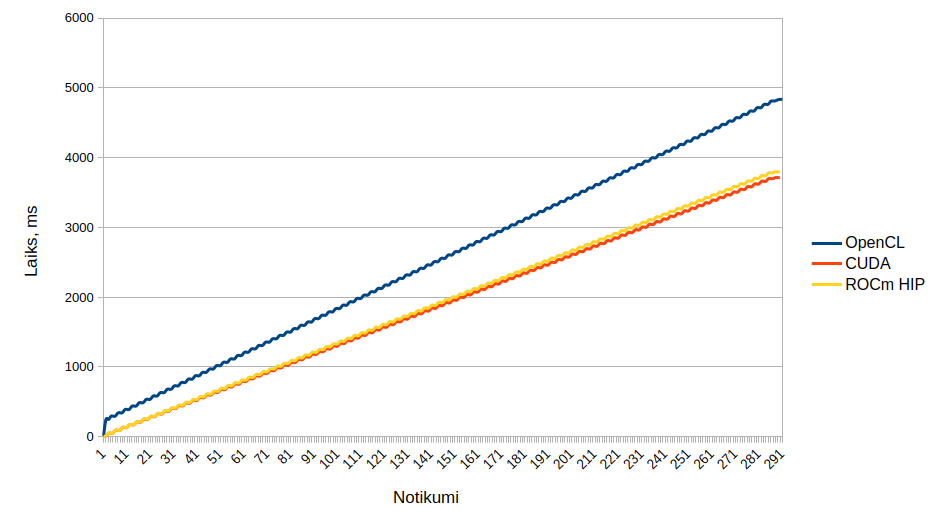
\includegraphics[width=\textwidth]{images/sha256_100m_not_found.png}
    \caption{Paroļu atguvēja izpildes laiki 100m parolēm (parole netika
    atrasta), datu straumes izmērs \( 2^{20} = 1048576\)}
    \label{img:sha256_100m_not_found_cum}
\end{figure}

\begin{figure}[H]
    \centering
    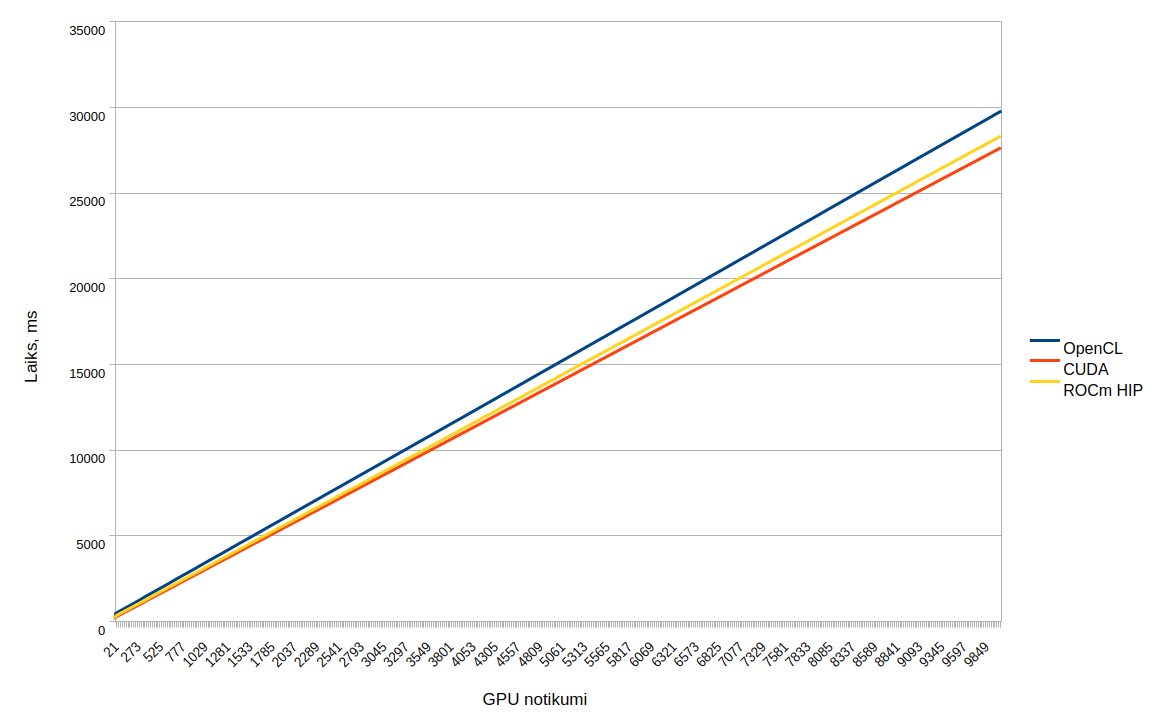
\includegraphics[width=\textwidth]{images/gol_10k_by_10k_10ksteps.png}
    \caption{10000x10000 Dzīves spēle ar 10000 soļiem}
    \label{img:gol_10k10k_10k_steps_cum}
\end{figure}

Pēc diagrammām var apstiprināt to, kas jau tika noskaidrots kursa darbā
saistībā ar CUDA un ROCm HIP - ROCm HIP ir neliela virsdarbe, salīdzinot ar
CUDA.\cite{kursa-darbs} Saistībā ar OpenCL platformu, katrs notikums ir,
relatīvi runājot, ar daudz lielāku virsdarbi.

Pēc jaunajiem etalonuzdevumiem var secināt, ka vidēji paroles atgūšanas
uzdevumā OpenCL ir par \(30.18\%\) lēnāks nekā CUDA un Dzīves spēles uzdevumā
par \(7.71\%\) lēnāks. Bet, salīdzinot HIP ar CUDA, AMD izstrādātā platforma ir
attiecīgi par \(2.25\%\) un \(2.47\%\) lēnāka.

Jāņem vērā, ka šie procenti iekļauj tikai kodolu izpildes laikus abos uzdevumu
gadījumos. Lai gan Dzīves spēlē lielākā uzdevuma daļa nodarbojas tieši tikai ar
kodolu izpildi (līdz ar to procentu starpība atbilst diagrammai), paroļu
atguvējā starp katra kodola izpildi notiek datu straumes apstrāde, kas iekļauj
datu ielasīšanu no faila, sagatavošanu GPGPU kodolam un datu pārsūtīšanu uz
videokarti, kas aizņem krietni lielāku laiku nekā paša kodola izpilde.

Ierēķinot kopējos programmu izpildes laikus (failu apstrāde), CUDA bija par
17\% ātrāka nekā ROCm HIP, un par 11\% ātrāka nekā OpenCL Dzīves spēles
uzdevumā, un attiecīgi 6\% ātrāka par ROCm HIP un 30\% ātrāka nekā OpenCL
paroļu atgūšanas uzdevumā. Abos gadījumos CUDA bija uzvarētāja, bet ROCm HIP un
OpenCL rezultāti dalījās.

Līdz ar to ir jāņem vērā CPU puses failu apstrādes virsdarbe, kura var
neparedzami ietekmēt mērījumus, jo pašu kodoli izpildes laiku mērijumi
konsekventi sarindo platformas.

Atsevišķi apskatot specifiskus GPGPU notikumus, starp platformām varētu atrast
kodolu izpildes nestabilitāti, tas ir, izpildes laiki varētu būt ļoti dažādi,
ar lielu variāciju, līdz ar to, ja apskata viena veida laidienu konfigurāciju
starp platformām kā izpildes laiku histogrammu, varētu noskaidrot cik stabila
ir kodolu izpilde.

Tā kā izmantotās videokartes (un CUDA, HIP platformu definētā) notikumu
precizitāte ir līdz \(\pm0.5\)\si{\micro\second}, histogrammas "spaiņa" (angļu
val. \textit{Histogram Bin}) platums noteikts kā \(10\)\si{\micro\second} - nav
pārāk šaura, lai nerastos kļūdas dēļ datu neprecizitātes, un nav pārāk plata, 
ka tiktu zaudēta izšķirtspēja. \cite{Freedman1981} No analizējamajiem datiem
izņemtas pašas pirmās kodolu izpildes programmu dzīves ciklā, kuras var saturēt
inicializācijas un kešatmiņas virsdarbes.

Līdzīgs risinājums izmantots priekš paroļu atguvēja žurnālfailu datiem, ar
papildus datu filtrēšanu, tā lai tiktu iekļautas tās kodolu izpildes, kuras
pilnībā aizņem visu datu straumes buferi, pretēji kodolu izpildes laiki var būt
neparedzami mainīgi.

\begin{figure}[H]
    \centering
    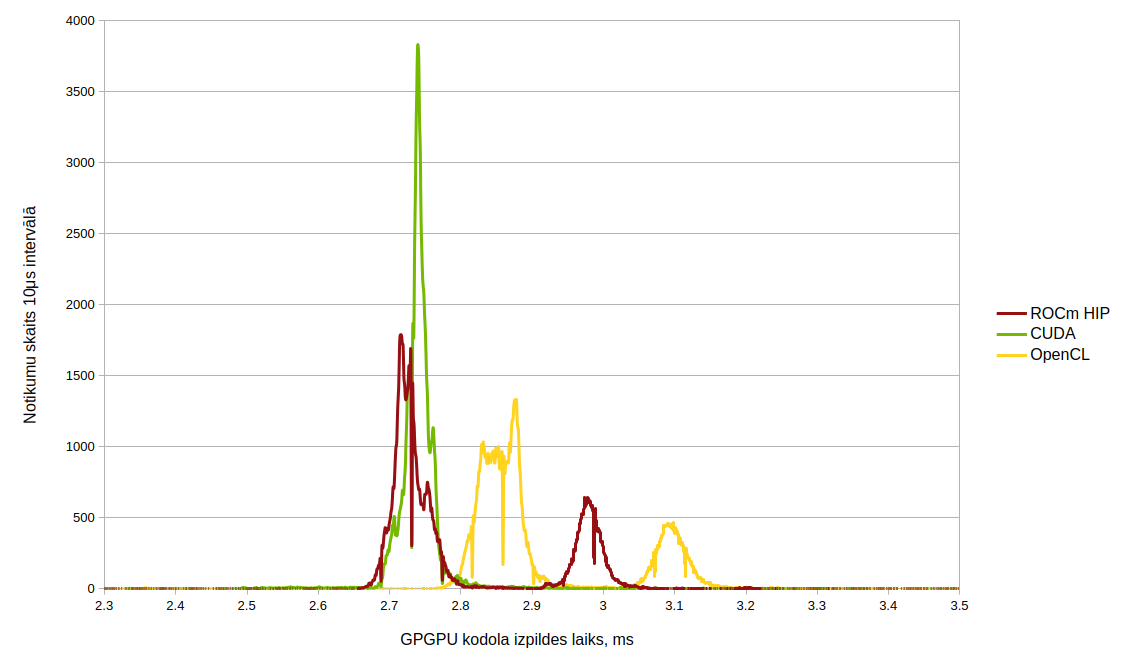
\includegraphics[width=\textwidth]{images/gol_distrib.png}
    \caption{Dzīves spēles kodolu izpildes histogramma (10000x10000 ar 10000 soļiem, 10 laidieni)}
    \label{img:gol_distrib}
\end{figure}


\begin{figure}[H] \centering
    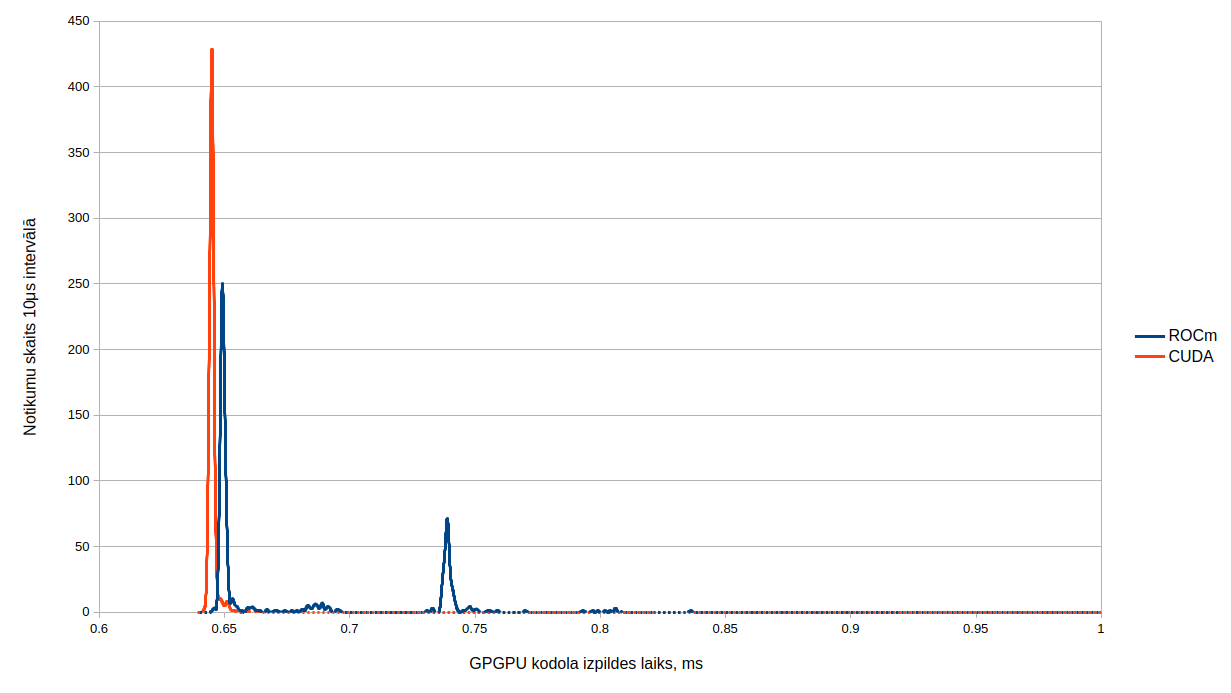
\includegraphics[width=\textwidth]{images/sha_distrib_cuda_rocm.png}
    \caption{Paroļu atguvēja izpildes histogramma CUDA un ROCm platformām (100
    000 000 paroles, 10 laidieni)} \label{img:sha_distrib}
\end{figure}


\begin{figure}[H] \centering
    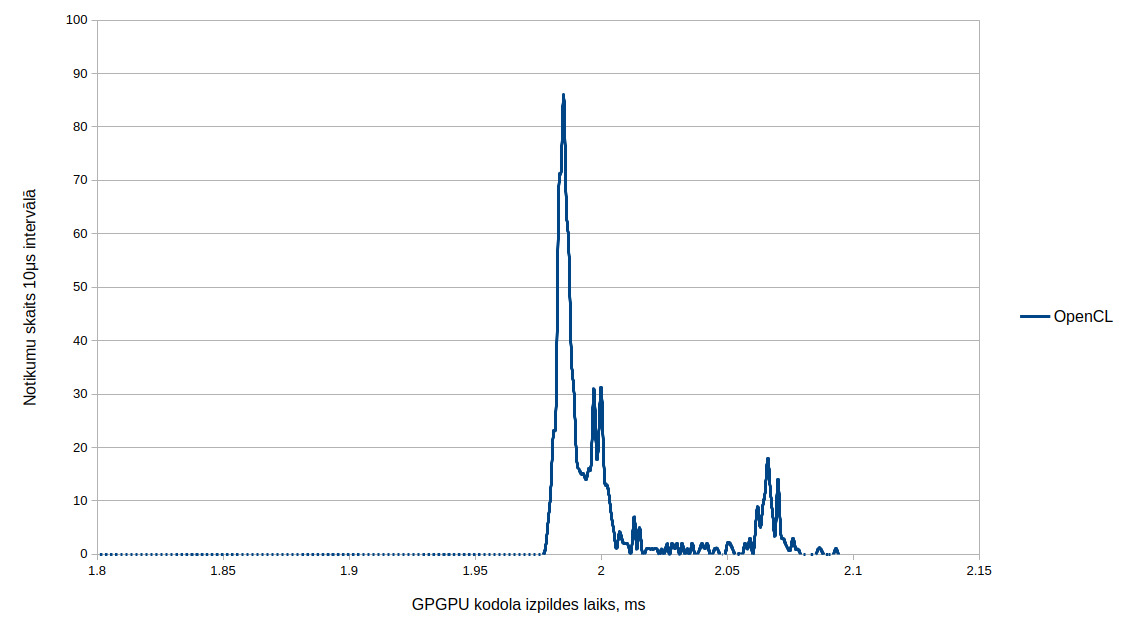
\includegraphics[width=\textwidth]{images/sha_distrib_opencl.png}
    \caption{Paroļu atguvēja izpildes histogramma OpenCL platformai (100 000
    000 paroles, 10 laidieni)} \label{img:sha_distrib_cl}
\end{figure}

Apskatot histogrammu bildes \ref{img:gol_distrib}, \ref{img:sha_distrib},
\ref{img:sha_distrib_cl}, var redzēt, ka mazākā izkliedētība ir CUDA
platformai. Pieņemot, ka dati veido normālo sadalījumu, tabulās \ref{tab:kern},
\ref{tab:kernel_exec_time_variations_gol} redzamas atbilstošās standartnovirzes
un variācijas.


\begin{table}[H]
    \centering
    \begin{tabular}{lrr}
    \hline
    \textbf{Platforma} & \textbf{Standartnovirze} & \textbf{Variāciju koeficients}\\ \hline
    CUDA    & 0.0015 & 0.0023 \\
    HIP     & 0.0408 & 0.0604  \\
    OpenCL  & 0.0275 & 0.0137 \\
    \hline
    \end{tabular}
    \caption{Platformu paroļu atguvēja kodolu izpildes laiku variācijas}
    \label{tab:kern} 
\end{table}


\begin{table}[H]
    \centering
    \begin{tabular}{lrr}
    \hline
    \textbf{Platforma} & \textbf{Standartnovirze} & \textbf{Variāciju koeficients}\\ \hline
    CUDA    & 0.1613 & 0.0587 \\
    HIP     & 0.1132 & 0.0405  \\
    OpenCL  & 0.1228 & 0.0422 \\
    \hline
    \end{tabular}
    \caption{Platformu Dzīves spēles kodolu izpildes laiku variācijas}
    \label{tab:kernel_exec_time_variations_gol} 
\end{table}


Interesants novērojums ir fakts, ka abos uzdevumu risinājumos HIP un
OpenCL izpildes laiku līknes satur divus pīķus ar diezgan līdzīgu
relatīvo attālumu starp šo pīķu modu. Datu analīzes laikā tika pieņemta
hipotēze, ka šo struktūru veido GPU aparatūras droselēšana.

Ja tā būtu, tad pie lielas noslodzes, kura laika ziņā ir palielināta HIP un OpenCL, varēja
iestāties aparatūras takts frekvences samazināšana, lai limitētu sistēmas
karšanu. Rezultātā veidojas divi pīķi - viens pie vienas takts frekvences un
viens pie otras.

Ja šī hipotēze būtu patiesa, tad varētu secināt, ka videokarte tika pietiekami
noslogota katra HIP un OpenCL laidiena laikā, kas radīja takts frekvences
mazināšanu. Tā kā uzdevumi, darbināmie kodoli ir pietiekami ekvivalenti, tad
palielinātais noslogojums pie pietiekami ekvivalentiem uzdevumiem,
salīdzinājumā ar CUDA, nosaka palielinātu neefektivitāti.

Pie tālakas analīzes tika secināts, ka hipotēze ir aplama, jo pie atkārtotas
manuālas etalonuzdevumu palaišanas netika novērota frekvences mazināšanās, un
videokartes temperatūra nepalielinājās līdz nedrošai robežai. Otrkārt, īstais
iemesls tika atklāts, apskatot secīgus individuālo laidienu kodolu izpildes
laikus (skatīt attēlus \ref{img:consecutive_kernel_exec_gol_cl}, \ref{img:consecutive_kernel_exec_gol_cuda}, \ref{img:consecutive_kernel_exec_gol_hip}).

\begin{figure}[H] \centering
    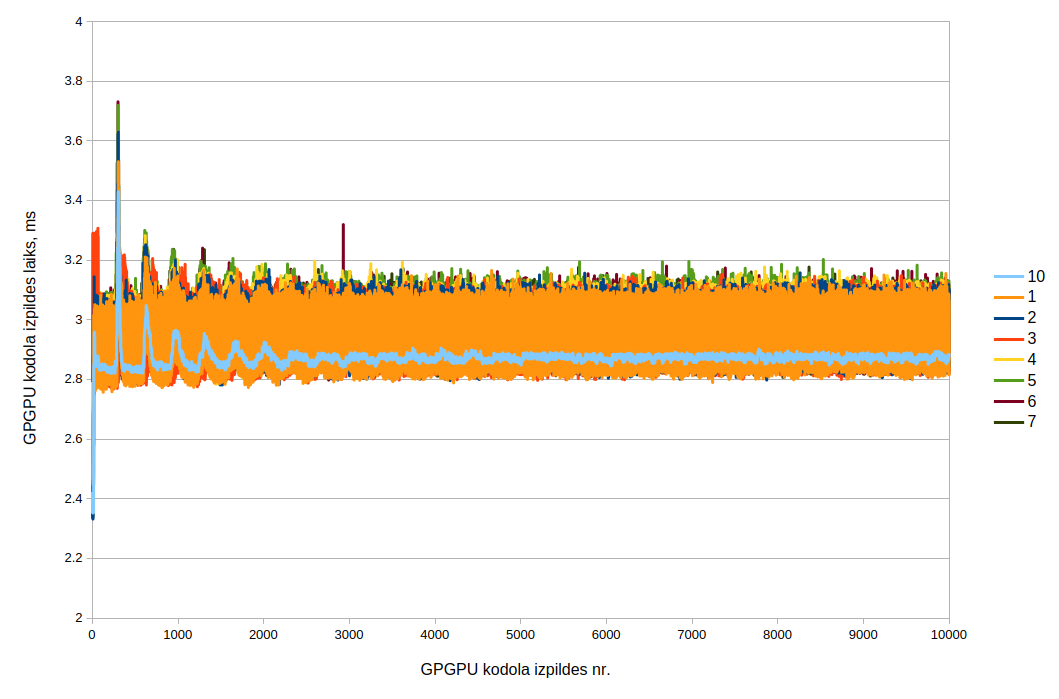
\includegraphics[width=\textwidth]{images/gol_opencl_consecutive_runs_10k_by_10k_10ksteps.png}
    \caption{Dzīves spēles secīgie atsevišķu laidienu izpildes laiks OpenCL
    platformā (10000x10000 ar 10000 soļiem)}
    \label{img:consecutive_kernel_exec_gol_cl}
\end{figure}


\begin{figure}[H] \centering
    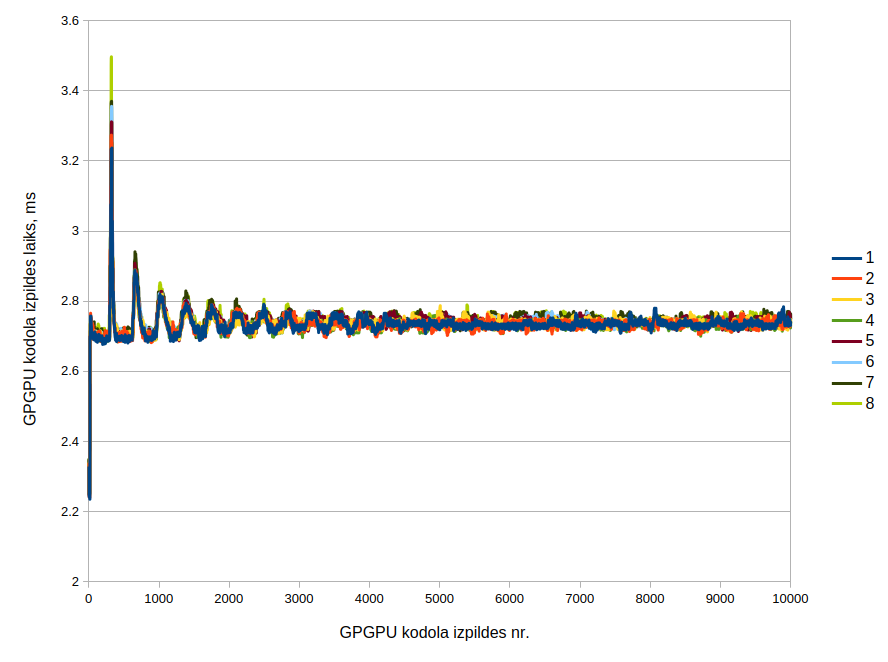
\includegraphics[width=\textwidth]{images/gol_cuda_consecutive_runs_10k_by_10k_10ksteps.png}
    \caption{Dzīves spēles secīgie atsevišķu laidienu izpildes laiks CUDA 
    platformā (10000x10000 ar 10000 soļiem)}
    \label{img:consecutive_kernel_exec_gol_cuda}
\end{figure}


\begin{figure}[H] \centering
    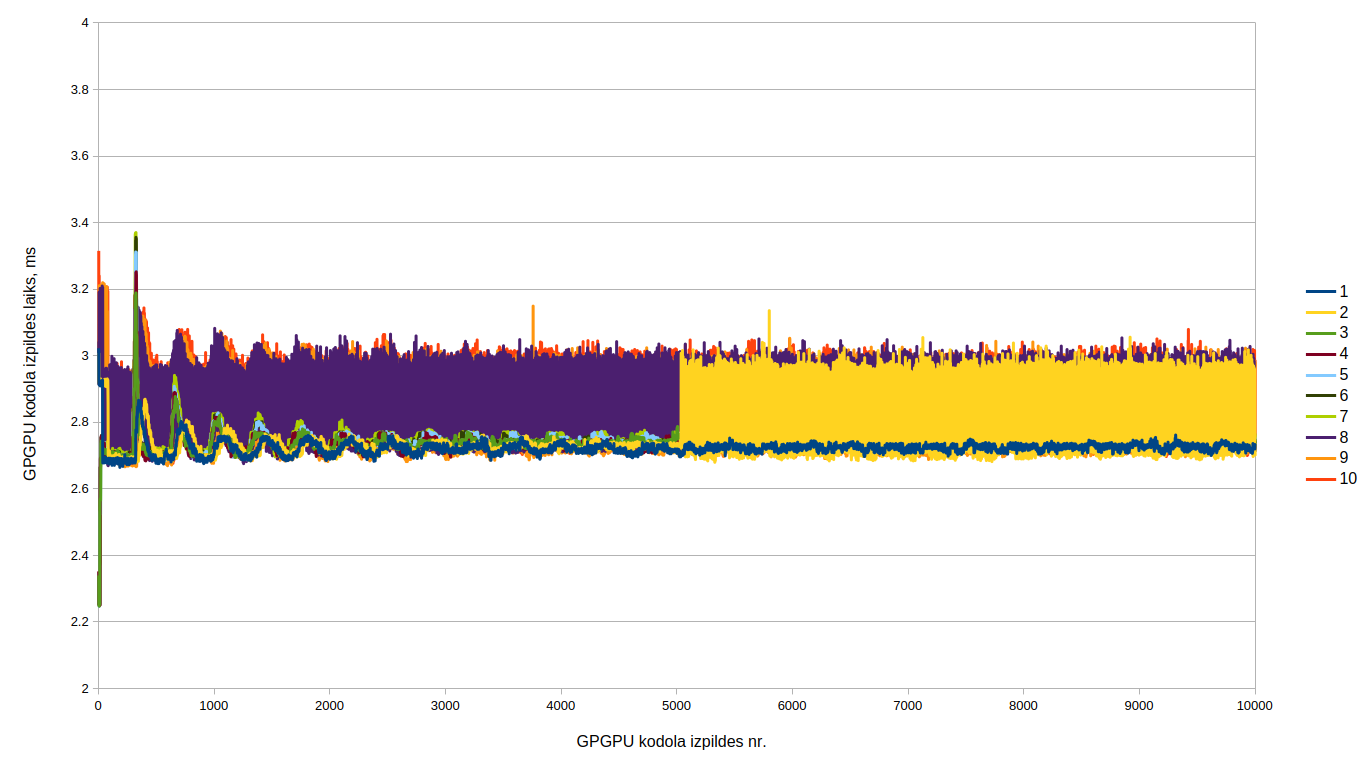
\includegraphics[width=\textwidth]{images/gol_hip_consecutive_runs_10k_by_10k_10ksteps.png}
    \caption{Dzīves spēles secīgie atsevišķu laidienu izpildes laiks ROCm HIP
    platformā (10000x10000 ar 10000 soļiem)}
    \label{img:consecutive_kernel_exec_gol_hip}
\end{figure}

Pēc diagrammām var secināt, ka visām platformām ir izteikta sākotnēja
svārstīšanās, kura norimst pēc vidēji 2800 kodolu izpildēm HIP platformai, 4400
CUDA un 2300 OpenCL. Pēc katras platformas individuālajām kodolu izpildes
laikiem katrai platformai tās ir 7731.7\si{\ms} HIP, 12087.8\si{\ms} CUDA un
6696.1\si{\ms} OpenCL (svārstību norimšanas laiki citām laidienu
konfigurācijām, protams, būs citādāki, minētie ir atbilstoši diagrammās
aprakstītajam). Bet jāņem vērā, ka HIP un OpenCL vairākos gadījumos ir izteikta
nerimstoša svārstīšanās, kura nav raksturīga nevienam CUDA laudienam starp
visām 10000x10000 konfigurācijām. 

Svārstīšanās izskaidrotu vairāku pīķu veidošanos histogrammās, bet pīķu
augstuma dažādība skaidrojama ar faktu, ka HIP un OpenCL nepārtrauktās
svārstības nav sinusoidālas. Ik pa laikam noteikti secīgu kodolu izpilde
ir relatīvi līdzīgi, līdz ar to viena veida vērtības, kuras laika ziņā ir
mazākās, ir izteikti biežāk (skatīt attēlu
\ref{img:consecutive_kernel_exec_gol_hip_cl_sample}).

\begin{figure}[H] \centering
    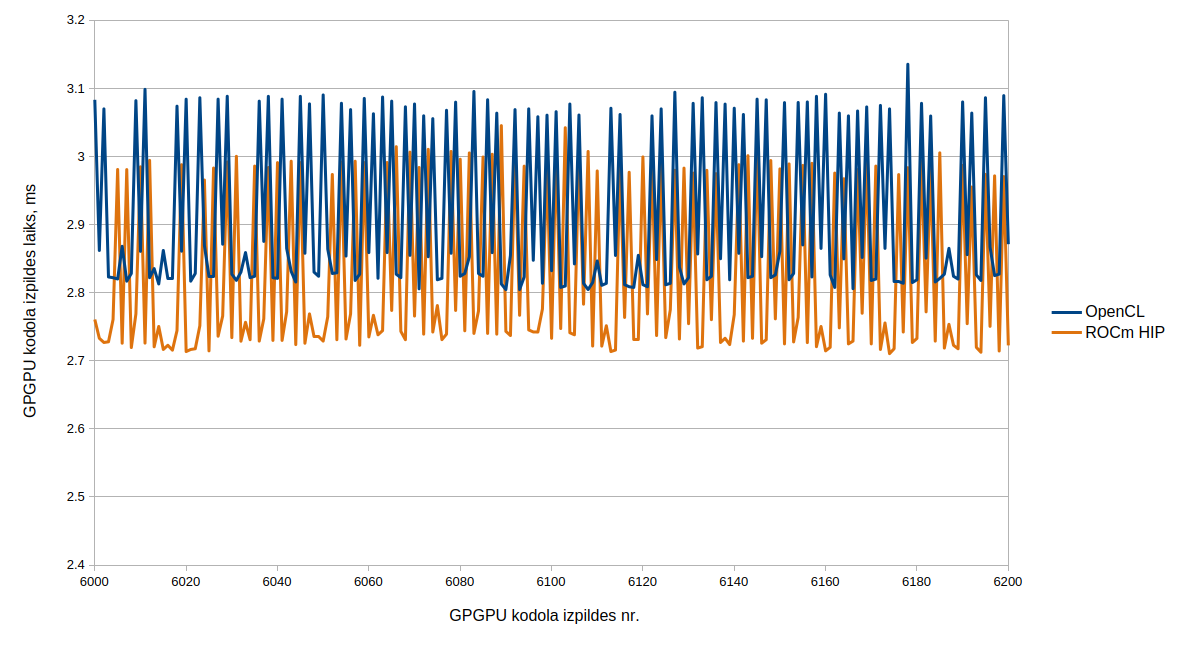
\includegraphics[width=\textwidth]{images/gol_hip_cl_sample_consecutive_runs_10k_by_10k_10ksteps.png}
    \caption{Dzīves spēles secīgie atsevišķu laidienu izpildes laiks ROCm HIP un CUDA
    platformā (10000x10000 ar 10000 soļiem)}
    \label{img:consecutive_kernel_exec_gol_hip_cl_sample}
\end{figure}

Līdzīgi ir arī ar paroļu atgūšanas mērijumiem, OpenCL un HIP risinājumiem ir
izteikta nepārtraukta svārstība, kas nav raksturīga CUDA (skatīt attēlus
\ref{img:sha_exec_cl}, \ref{img:sha_exec_cuda}, \ref{img:sha_exec_hip}).

\begin{figure}[H] \centering
    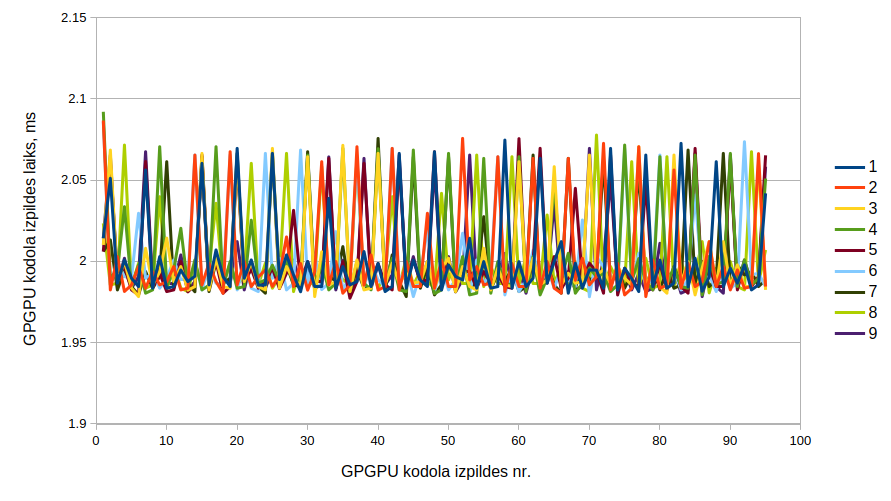
\includegraphics[width=\textwidth]{images/sha_kernel_exec_cl.png}
    \caption{OpenCL paroļu atguvēja kodola izpildes laiki}
    \label{img:sha_exec_cl}
\end{figure}

\begin{figure}[H] \centering
    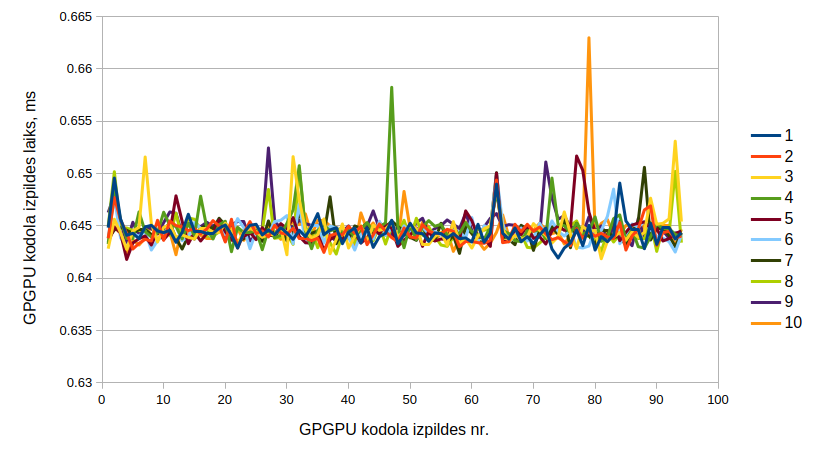
\includegraphics[width=\textwidth]{images/sha_kernel_exec_cuda.png}
    \caption{CUDA paroļu atguvēja kodola izpildes laiki}
    \label{img:sha_exec_cuda}
\end{figure}

\begin{figure}[H] \centering
    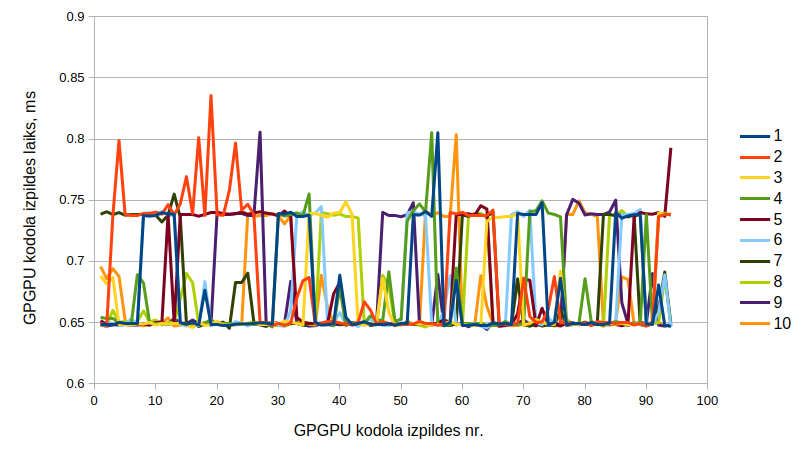
\includegraphics[width=\textwidth]{images/sha_kernel_exec_hip.png}
    \caption{HIP paroļu atguvēja kodola izpildes laiki}
    \label{img:sha_exec_hip}
\end{figure}


Atlikusī mērāmā GPU puses atšķirība starp uzdevumiem ir nepieciešamību
iteratīvi sagatovot atmiņu un to piepildīt ar straumētajām parolēm paroļu
atguvēja uzdevumā. Dzīves spēles uzdevumā šie buferi praktiski netiek aiztikti,
jo izejas režģa buferi var atkārtoti lietot kā ieejas, un otrādi ar ieejas
buferi. Paroļu atguvējam nepieciešams ielasīt jaunus datus visu laiku, līdz ar
to, pirms katras kodola izpildes tiek sūtīti dati uz VRAM.
Šādos mērījumos nav saskatāmas nepārtrauktas svārstības (skatīt attēlus
\ref{img:sha_buf_creation_cl}, \ref{img:sha_buf_creation_cuda},
\ref{img:sha_buf_creation_hip}).


\begin{figure}[H] \centering
    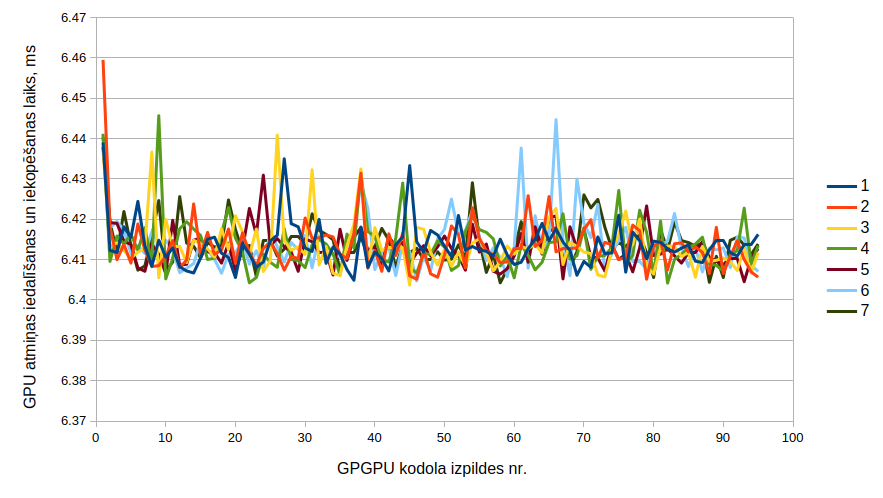
\includegraphics[width=\textwidth]{images/sha_buf_creation_cl.png}
    \caption{OpenCL paroļu atguvēja atmiņas iedalīšana un aizpildīšana}
    \label{img:sha_buf_creation_cl}
\end{figure}


\begin{figure}[H] \centering
    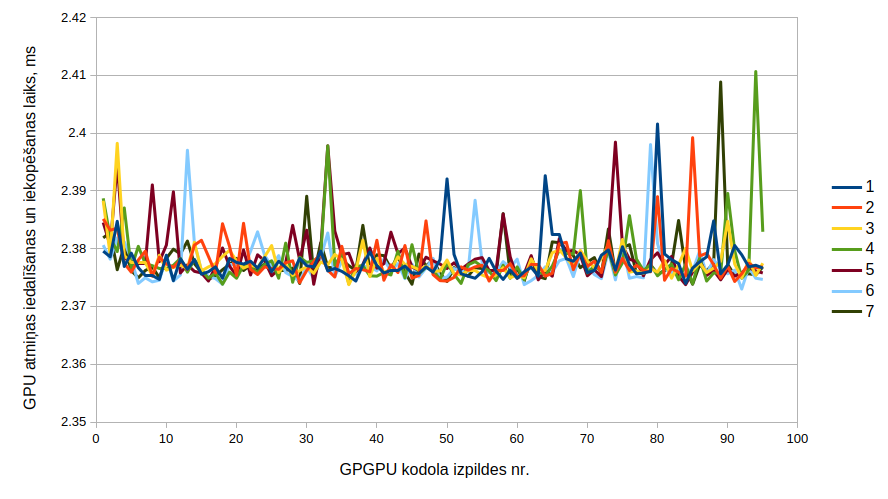
\includegraphics[width=\textwidth]{images/sha_buf_creation_cuda.png}
    \caption{CUDA paroļu atguvēja atmiņas iedalīšana un aizpildīšana}
    \label{img:sha_buf_creation_cuda}
\end{figure}


\begin{figure}[H] \centering
    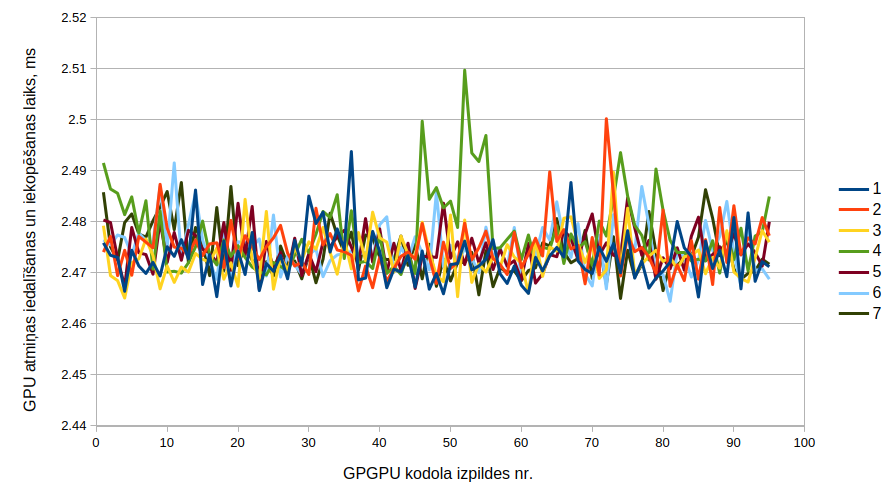
\includegraphics[width=\textwidth]{images/sha_buf_creation_hip.png}
    \caption{ROCm HIP paroļu atguvēja atmiņas iedalīšana un aizpildīšana}
    \label{img:sha_buf_creation_hip}
\end{figure}

Lai gan izskatās, ka izmērītie laiki ir diezgan haotiski un ar lielu amplitūdi
visās trīs platformās, jāņem vērā visās trīs diagrammās Y laika ass solis ir
10\si{\micro\second}, turpretī, kodola izpildē tās ir 50\si{\micro\second}.
Tabulā \ref{tab:amplitudas} redzams abu mērījumu amplitūdu salīdzinājums.
Pēc to datiem var secināt, ka OpenCL un HIP atmiņas apstrādes laika variācijai
ir mazāka kopējā ietekme uz kodola izpildes laiku, jo kodola izpildes laika
variācija ir lielāka. Bet CUDA gadījumā ir redzams pretējais - atmiņas apstrādes
variācijai tomēr ir lielāka ietekme.

\begin{table}[H]
    \centering
    \caption{Paroļu atguvēja GPGPU kodolu izpildes un atmiņas izveides,
    pārsūtīšanas amplitūdu salīdzinājums}
\label{tab:amplitudas}
\begin{tabular}{rrrr}
    Platforma & Kodola izpildes amplitūda, ms & Atmiņas amplitūda, ms& \% \\ \hline
OpenCL & 0.1147 & 0.0558 & 48.65\% \\
CUDA & 0.0212 & 0.0376 & 177.36\% \\
ROCm HIP & 0.1911 & 0.0453 & 23.70\% \\
\hline
\end{tabular}
\end{table}
